\chapter{Inertia}\label{app:Inertia}
One set of parameters in the model is the inertia of the quadcopter around its axes, roll, pitch and yaw. There are different approaches to find the inertia, but to get a good starting point the quadcopter is split op in several masses and the inertia is found analytically.

The quadcopter is first decomposed to a set of objects for which the inertia is well defined, this is done in \autoref{fig:quadcopterMasses}.

\begin{figure}[H]
  \centering
  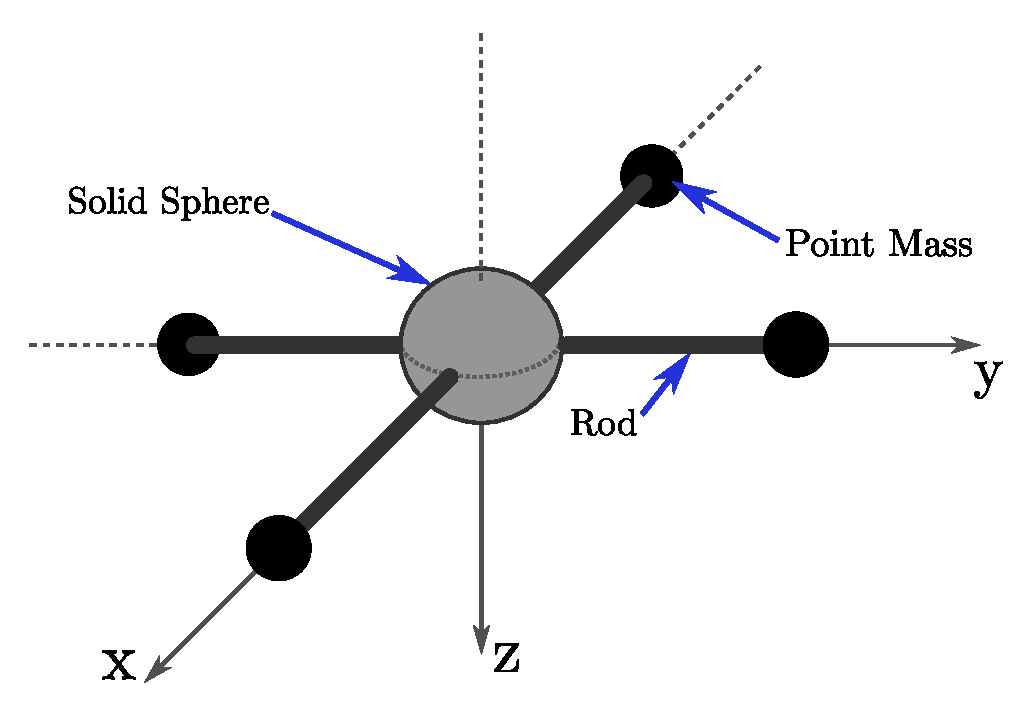
\includegraphics[width=.6\linewidth]{figures/quadcopterMasses}
  \caption{The quadcopter with attached hardware as given.}
  \label{fig:quadcopterMasses}
\end{figure}

The inertia must be calculated around the axes on which the quadcopter will turn. Since the quadcopter is controlled in plus configuration, the inertia is calculated around the x-, y- and z-axis.

The objects are analyzed individually around the center of mass, CM, see \autoref{fig:inertiaObjects}, after which the inertias are summed for each axis of rotation.

\begin{figure}[H]
  \centering
  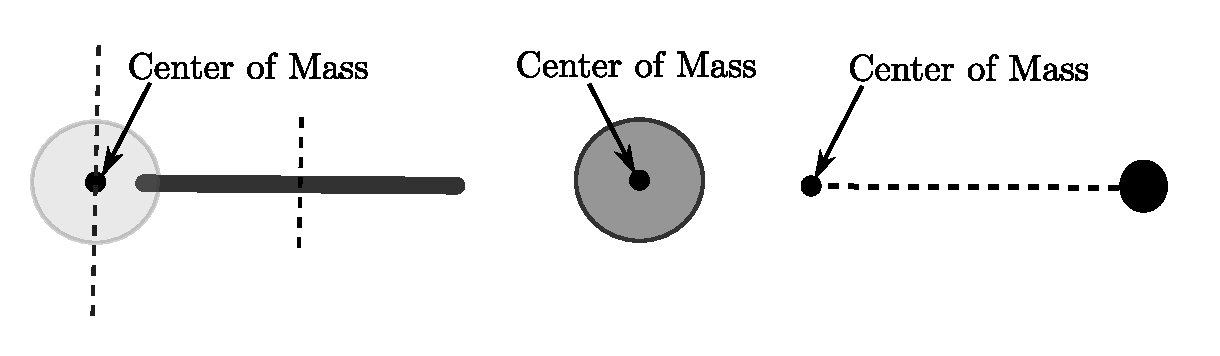
\includegraphics[width=.9\linewidth]{figures/inertiaObjects}
  \caption{The quadcopter with attached hardware as given.}
  \label{fig:inertiaObjects}
\end{figure}

To calculate the inertias it is necessary to distribute the mass of the quadcopter between the decomposed objects in \autoref{fig:quadcopterMasses}. To do this the motor and propeller was weighed and considered to be the point mass, then the arm and ESC was weighed and considered to be the rod. Finally the entire quadcopter was weighed and the weight of the other objects subtracted to find the mass of the sphere.

The inertia of the sphere is directly given by
\begin{flalign}
  I_s &= \frac{2}{5}  m_s r_s^2    \unit{kg \cdot m ^2}
\end{flalign}
%
\begin{where}
  \va{I_s}  {is the moment of inertia around the CM of the quadcopter}  {kg \cdot m ^2}
  \va{m_s}  {is the mass of the sphere}  {kg}
  \va{r_s}  {is the radius of the sphere}  {m}
\end{where}

Plugging the measured quantities into the formula yields the following

%\begin{flalign}
%  I_s &= \frac{2}{5}  m_s r_s^2    \unit{kg \cdot m ^2}
%\end{flalign}

For a point mass the moment of inertia around the CM of the quadcopter is given by
\begin{flalign}
  I_p &= m_p d_p ^2   \unit{kg \cdot m ^2}
\end{flalign}
%
\begin{where}
  \va{I_p}  {is the moment of inertia around the CM of the quadcopter}  {kg \cdot m ^2}
  \va{m_p}  {is the mass of the point}  {kg}
  \va{d_p}  {is the distance from the point mass to the CM of the quadcopter}  {m}
\end{where}

To calculate the moment of inertia of the rod, it is first evaluated around its own axis, see \autoref{fig:inertiaObjects}. Then by use of the parallel axis theorem the inertia can be moved, such that it is described around the center of mass of the quadcopter.

The parallel axis theorem states that any mass with known inertia around its own center of mass can be described around a parallel axis by adding its mass multiplied by the distance, between the parallel axes, squared. For the rod this yields the following
\begin{flalign}
  I &= \frac{1}{12}  m_r L_r ^2  + m_r d_r^2  \unit{kg \cdot m ^2}
\end{flalign}
%
\begin{where}
  \va{I_r} {is the moment of inertia around CM of the rod}  {kg \cdot m ^2}
  \va{m_r} {is the mass of the rod}  {kg}
  \va{L_r}   {is the length of the rod}  {m}
  \va{d_r}   {is the distance from CM of the rod to the CM of the quadcopter}{m}
\end{where}